We describe the full architecture of our system.

%TC:ignore
\begin{figure}[H]
    \centering
    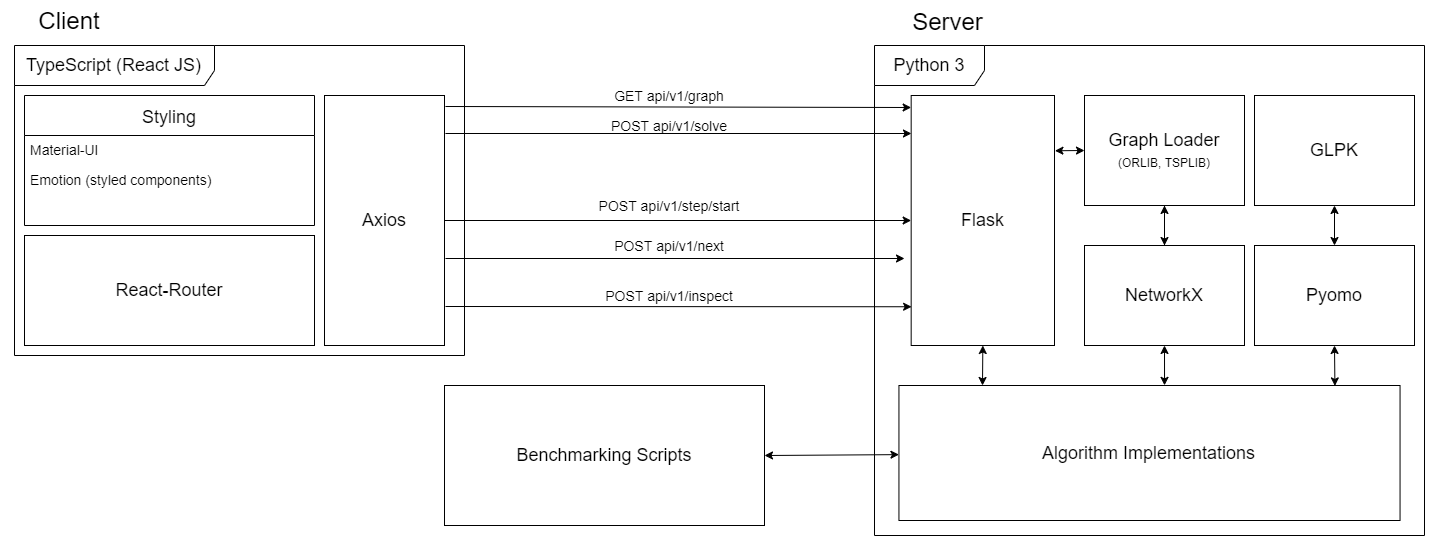
\includegraphics[width=\textwidth]{images/system_architecture.png}
    \caption{System Architecture}
    \label{fig:system_architecture}
\end{figure}
%TC:endignore

\subsubsection{Solver Flow}
The solution visualisation flow contains a single request:
%TC:ignore
\begin{figure}[H]
    \centering
    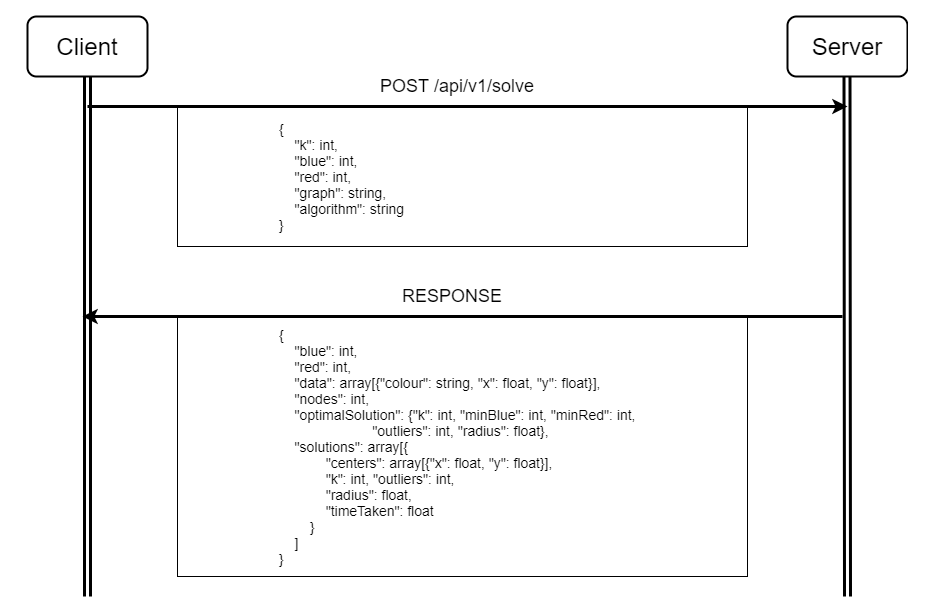
\includegraphics[width=0.7\textwidth]{images/solver_ui/post_solve_flow.png}
    \caption{Solve Request}
    \label{fig:solve_request}
\end{figure}
%TC:endignore

\subsubsection{Stepped Solver Flow}
The stepped solver is a multi request flow; it is initialised through the '/start' endpoint which creates a solver iterator and returns a UUID token. The solver iterator is implemented using a Python generator function which allows us to use lazy evaluation to only get the next required step.
%TC:ignore
\begin{figure}[H]
    \centering
    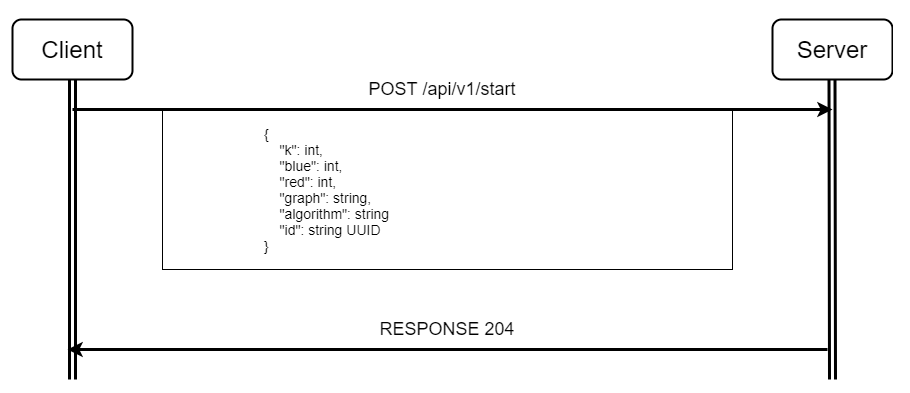
\includegraphics[width=0.7\textwidth]{images/stepped_solver_ui/start_stepped_flow.png}
    \caption{/api/v1/start flow}
    \label{fig:stepped_start_request}
\end{figure}
%TC:endignore

Subsequent calls to the '/next' and '/inspect' endpoints with the UUID is used to exhaust the iterator. Inspect moves to the next chronological step and next skips to the next major step.
%TC:ignore
\begin{figure}[H]
    \centering
    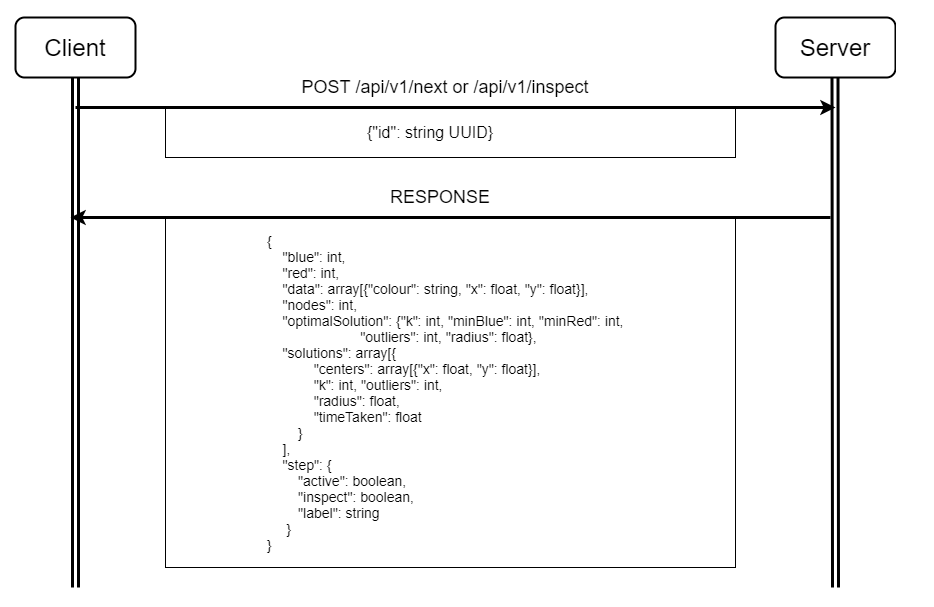
\includegraphics[width=0.7\textwidth]{images/stepped_solver_ui/next_inspect_stepped_flow.png}
    \caption{/api/v1/next and /api/v1/inspect flow}
    \label{fig:stepped_next_inspect_request}
\end{figure}
%TC:endignore

%\subsubsection{Build and Deployment}
%Following the accessibility requirement, we also consider the ease of setup. As we use linear program solvers, this is an extra dependency that is not installable the dependency manager Python pip. Therefore we use Docker, we configure the build file to create and package the static web files, install all dependencies; a user can clone our git repository, execute 'docker build' and 'docker run', then have a working instance of our application. This also allows us to easily deploy to cloud platforms such as Heroku.